\documentclass[11pt]{article}

\usepackage{physics}
\usepackage[top=1in, bottom=1in, left=0.5in, right=0.5in]{geometry}
\usepackage{hanging}
\usepackage{amsfonts, amsmath, amssymb}
\usepackage[none]{hyphenat}
\usepackage{fancyhdr}
\usepackage[nottoc, notlot, notlof]{tocbibind}
\usepackage{graphicx}
\graphicspath{{./images/}}
\usepackage{float}
\usepackage{siunitx}
\usepackage{esint}

\pagestyle{fancy}
\fancyhead{}
\fancyfoot{}
\fancyhead[L]{MAP2302 Professor Jury}
\fancyhead[R]{Sai Sivakumar 10/28/20}
\fancyfoot[R]{\thepage}
\renewcommand{\headrulewidth}{0pt}

\setlength{\parindent}{0cm}
\setlength{\parskip}{5pt}
\renewcommand{\baselinestretch}{1.25}

\newcommand{\ihat}{\boldsymbol{\hat{\textbf{\i}}}}
\newcommand{\jhat}{\boldsymbol{\hat{\textbf{\j}}}}
\newcommand{\dr}{\vec{r}~^{\prime}(t)}
\newcommand{\dx}{x^{\prime}(t)}
\newcommand{\dy}{y^{\prime}(t)}

\newcommand{\br}[1]{\left(#1\right)}
\newcommand{\sbr}[1]{\left[#1\right]}
\newcommand{\cbr}[1]{\{#1\}}

\newcommand{\dprime}{\prime\prime}

\usepackage{mathtools}

\DeclarePairedDelimiterX{\abr}[1]{\langle}{\rangle}{#1}

\setcounter{page}{1}

\begin{document}

Section 4.8: 7, 8, 9, 10, 
Section 4.9: 11, 
Section 4.10: 3, 
Section 5.2: 13, 29

Section 4.8 \\

7. 

(a) The tangential velocity of the mass is given by multiplying the angular velocity times the distance from the axis of rotation, so $\ell \omega  = \ell \theta^{\prime}$. Then the linear momentum will be given as $m\ell \theta^{\prime}$

The magnitude of the angular momentum of the mass is given by the product of the lever arm length times the magnitude of the linear momentum. Since the linear momentum is tangential to the path taken by the mass, it is normal to the lever arm and so it is apparent that the angular momentum is equal to $m\ell^2\theta^{\prime}$.

(b) The torque then is the product of the lever arm length and the component of gravity normal to the lever arm vector. Gravity is a restoring force in the case of the pendulum, so the force $mg\sin(\theta)$ will always act against the direction of motion, so we can give it as $-mg\sin(\theta)$, and then the torque is then just $-\ell mg\sin(\theta)$.

(c) Newton's law of rotational motion states that the rate of change of angular momentum is equal to torque. Then $\br{m\ell^2\theta^{\prime}}^{\prime} = -\ell mg\sin(\theta) \to m\ell^2\theta^{\dprime} = -\ell mg\sin(\theta) \to m\theta^{\dprime} + m\frac{g}{\ell}\sin(\theta) = 0$. \\

8. Using the energy integral lemma, it is apparent that we can represent the energy of the system as: $$E = \frac{1}{2}m\br{\theta^{\prime}}^2-m\frac{g}{\ell}\cos(\theta)$$

Differentiating both sides we can find that the energy is a constant: $$E^{\prime} = m\theta^{\prime}\theta^{\dprime} + m\frac{g}{\ell}\sin(\theta)\theta^{\prime} = \theta^{\prime}\br{m\theta^{\dprime} + m\frac{g}{\ell}\sin(\theta)} = 0$$ 

Hence energy is a constant.\\

9. We seek to find an initial velocity such that the pendulum travels from the lowest position $\theta = 0$ to just before $\theta = \pi$. This is accomplished by equating the energy at the peak (where velocity should be 0) and with the energy at the initial position.
$$\frac{1}{2}m\br{0}^2-m\cos(\pi) = \frac{1}{2}m\br{\theta^{\prime}(0)}^2-m\cos(0) \to \theta^{\prime}(0) = \pm 2$$

Hence we can give the mass an initial angular velocity of $2$ radians per second in either the clockwise or counterclockwise direction to achieve almost reaching the apex.\\

10. Since the initial conditions are $\theta(0) = \alpha,~ \theta^{\prime}(0) = 0$, we can substitute them into the energy equation for all $t$ (energy is constant):
$$E = \frac{1}{2}m\br{0}^2-m\frac{g}{\ell}\cos(\alpha) = -m\frac{g}{\ell}\cos(\alpha)$$ 

Because the energy is bounded, the term containing $\theta(t)$ will always be bounded above by that energy (remember $\alpha$ is positive and less than $\pi$).
$$-m\frac{g}{\ell}\cos(\theta(t)) \leq -m\frac{g}{\ell}\cos(\alpha) \to \arccos(\cos(\theta(t))) = \arccos(\cos(\alpha)) $$

By definition of the inverse of cosine, we have $\abs{\theta(t)} \leq \abs{\alpha} \to \abs{\theta(t)} \leq \alpha$. \\

Section 4.9 \\

11. The IVP modeling this scenario is given by $$1y^{\dprime} + 0.2y^{\prime} + 100y = 0, ~y(0) = 0, ~y^{\prime}(0) = 1$$ and the solution is found by finding the first $t_0$ such that the $y^{\prime}(t_0)$ vanishes.

The roots of the associated quadratic of differential operators are $\frac{-1}{10}\pm i\frac{3\sqrt{1111}}{10}$, so the general solution is given by $$y = c_1e^{\frac{-1}{10}t}\sin(\frac{3\sqrt{1111}}{10}t) + c_2e^{\frac{-1}{10}t}\cos(\frac{3\sqrt{1111}}{10}t)$$ and then use the initial data to find that the particular solution is: $$y = \frac{10}{3\sqrt{1111}}e^{\frac{-1}{10}t}\sin(\frac{3\sqrt{1111}}{10}t)$$

So the first derivative is $$y^{\prime} = \br{-\frac{1}{3\sqrt{1111}}e^{\frac{-1}{10}t}\sin(\frac{3\sqrt{1111}}{10}t)+e^{\frac{-1}{10}t}\cos(\frac{3\sqrt{1111}}{10}t)}$$ which vanishes at $t = \frac{10\arctan(3\sqrt{1111})}{3\sqrt{1111}}$. \\

\newpage

Section 4.10 \\

3. Because the linear differential operator $\sbr{D^2+9}$ also annihilates $2\cos(3t)$, we have roots $\pm 3i$ in multiplicity $2$ each, so the general equation of motion is given by $y= c_1\sin(3t) + c_2\cos(3t) + c_3t\sin(3t) + c_4t\cos(3t)$, which after determining the coefficients by putting this back into the differential equation becomes $y= c_1\sin(3t) + c_2\cos(3t) + \frac{1}{3}t\sin(3t)$.

The initial data is used to find the other two coefficients, so the final equation of motion becomes:
$$y = \cos(3t) + \frac{1}{3}t\sin(3t)$$

The behavior initially looks like the cosine term, but then its contribution to the graph is made negligble as the sine term grows larger. (the frequency approaches that of the sine term, initially it may be slower just due to the summation of terms of around equal contribution)

\begin{figure}[h]
    \centering
    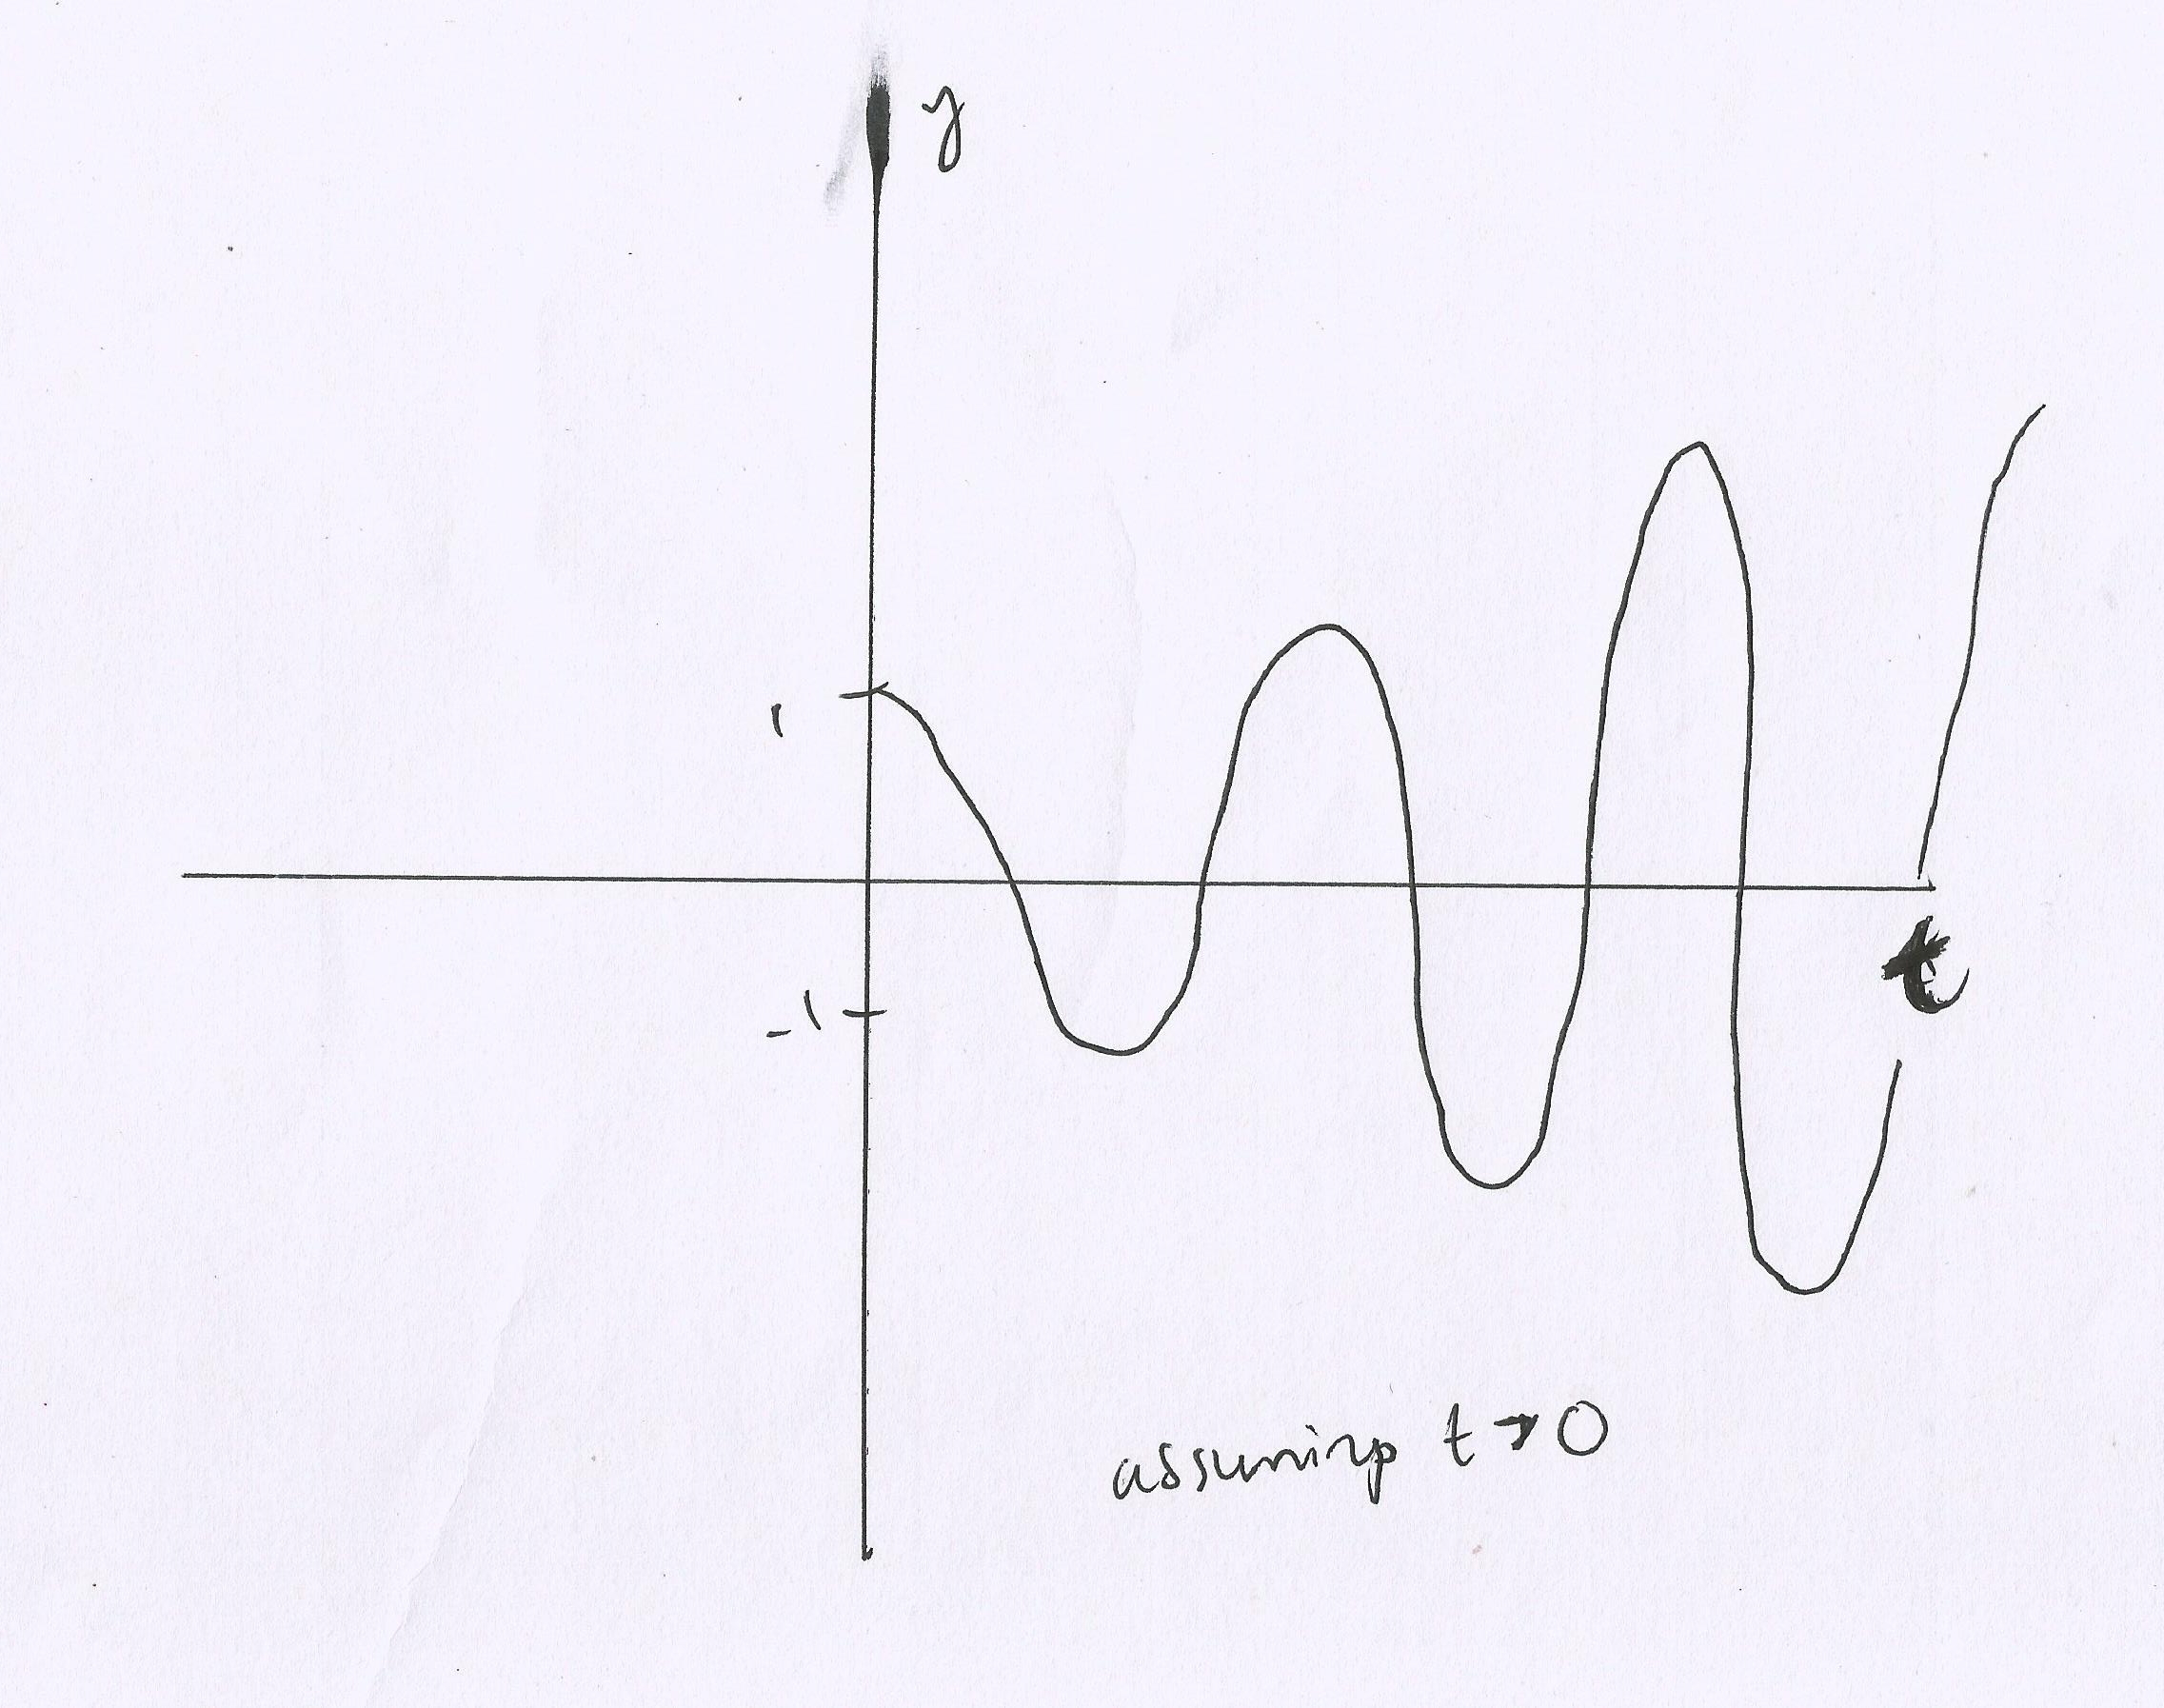
\includegraphics[scale=0.5]{graph}
\end{figure}

Section 5.2 \\

13. Rearrange the equations and apply the differential operator $(D-1)$ to the second equation to find the system:

$$\br{D-1}x = -4y$$
$$\br{D-1}^2y = \br{D-1}x$$\

We can subtract the top equation from the bottom one to find the following differential equation:
$$\br{D^2-2D+5}y = 0$$

This has a general solution given by $y = c_1e^t\sin(2t) + c_2e^t\cos(2t)$, and we can use this in the original second equation $y^{\prime} = x+y$ to immediately find $x = 2c_1e^t\cos(2t) - 2c_2e^t\sin(2t)$.\\

29. We can eliminate within the system by multiplying the first equation through by the differential operator $\br{D-1}$.

We should obtain the following system using differential operators after some shuffling:

$$\br{D-1}\br{D-\lambda} = -\br{D-1}y$$
$$3x = \br{D-1}y$$

Eliminate the y term by adding both equations together (eliminating x instead via a different process brings us to the same result) and rearrange the differential terms to get a quadratic of differential operators.
$$\br{D^2-(\lambda + 1)D + (\lambda + 3)}x = 0$$

We desire roots to have a real part that is negative so that we have a function that is going to be shrinking and thus bounded (has exponential decay terms).

Via Vieta's formulas we know the roots $r_1,~ r_2$ have to satisfy the following equations:

$$r_1+r_2 = 1+\lambda$$
$$r_1r_2 = \lambda+3$$

Since we have both roots as negative, then the right hand side of the first equation must be negative, meaning $\lambda < 1$. Similarly the product should be a positive number, so $\lambda > -3$. Thus the solution curve for $y$ or $x$ is bounded so long as $\lambda \in \br{-3,-1}$.

\end{document}